%
%
%


\begin{frame}[t,allowframebreaks]{Basic structure of a Convolutional Neural Network -}

    The \index{CNN}\index{convolutional neural network}\gls{cnn} 
    input data (typically, an image) is a {\bf 3-D grid structure}
    that has {\it height}, {\it width} and {\it depth}:
    \begin{itemize}
        \item Two dimensions are devoted to {\bf spatial information}
        \item The third dimension stores {\bf independent properties} of each pixel
        \begin{itemize}
            \item For example, the {\bf intensities of the three primary colours}
             (red, green, and blue) that help us encode the precise colour of the pixel.
        \end{itemize}
    \end{itemize}

    \begin{columns}
        \begin{column}{0.22\textwidth}
            \vspace{0.0cm}
            \begin{center}
                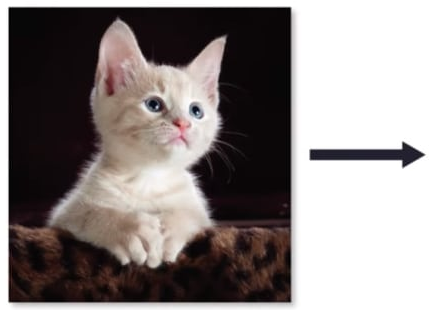
\includegraphics[width=1.0\textwidth]
                    {./images/cnn/example_inputs/example_1_cat.png}\\
            \end{center}
        \end{column}
        \begin{column}{0.46\textwidth}
            \vspace{0.0cm}
            \begin{center}
                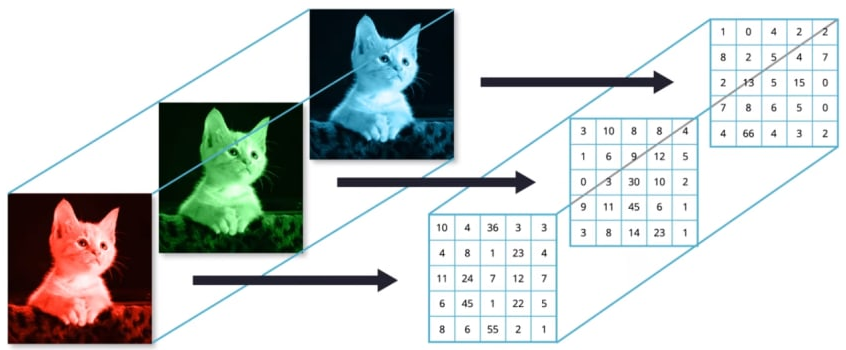
\includegraphics[width=1.0\textwidth]
                  {./images/cnn/example_inputs/example_1_cat_rgb.png}\\
            \end{center}      
        \end{column}
        \begin{column}{0.32\textwidth}
            \vspace{0.0cm}
            \begin{center}
                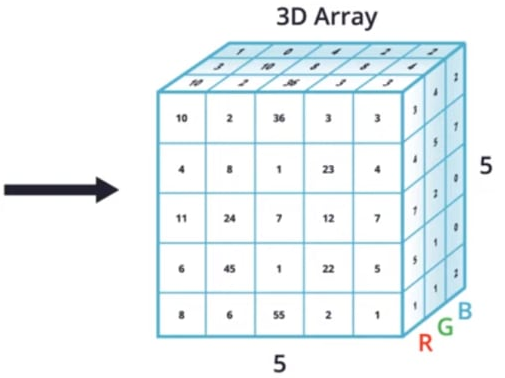
\includegraphics[width=1.0\textwidth]
                  {./images/cnn/example_inputs/example_1_cat_array.png}\\
            \end{center}      
        \end{column}
    \end{columns}
    \begin{center}
        {\scriptsize 
        \color{col:attribution} 
        Image adapted from \cite{DevCommunity:GoingFurtherWithCNN}.}\\
    \end{center}      

    \framebreak

    A \index{CNN}\index{convolutional neural network}\gls{cnn} consists of {\bf several layers}

    \begin{itemize}
        \item
            Like in traditional \index{feed forward}\glshyph{feed forward} neural networks, 
            and each layer processes information produced at the layer that precedes it.
        \item
            Typically, {\bf three types of layers}:
            \index{convolution}\gls{convolution}, 
            \index{pooling}\gls{pooling} and 
            \index{ReLU}\gls{relu}.
        \item
            Connections are sparse, though the latter part can be fully connected.
        \item
            {\bf Spatial relationships are preserved} between layers
    \end{itemize}

    \begin{center}
        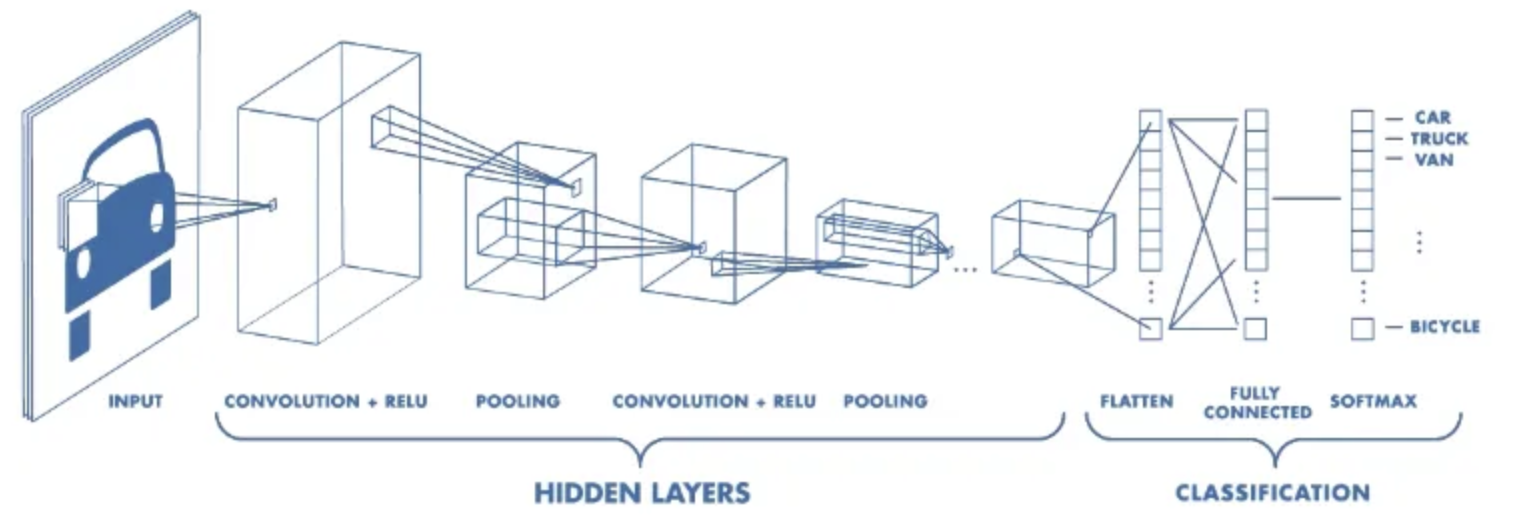
\includegraphics[width=0.8\textwidth]
          {./images/cnn/basic_structure/chatterjee19_classic_cnn_architecture.png}\\
        {\scriptsize 
          Classic CNN architecture.
          \color{col:attribution} 
          Image from \cite{TowardsDataScience:BasicsOfClassicCNN}}\\    
    \end{center}      
   
\end{frame}
